\chapter{基于最优控制理论的群决策算法}
在上一章中,文章讨论了如何运用最优控制的相关理论,在不同的约束条件下给出控制量的具体形式。但这些情形只是针对一辆CAV的控制策略。要进行群决策,还需要其他的算法辅助,例如通过路口顺序的决策算法,以及整个系统在状态改变时,一部分车所处的情景可能改变,需要对其重新运行单车的最优控制算法。

\section{通行序列决策}
前文一直假设已经得到了某种序列$\mathcal{N}(t)$,然后根据该序列迭代的确定达到交汇口时间$t_\mathrm{m}$的下界。这一节讨论如何确定该通行顺序。

关于路口通行顺序的确定,已经有大量的研究工作。这些顺序不仅用于道路交汇口,也用于交叉口(十字路口等)的通行顺序确定。常用的一些顺序有:
\begin{itemize}
\item \textbf{先进先出(FIFO)}\ \ 按照进入控制区的时间先后通过路口,先进入的优先通过。文献\cite{Kim2013Collision,Azimi2011Vehicular}中即使用了这种通行顺序进行控制。
\item \textbf{与路口的距离}\ \ \ 文献\cite{Fankhauser2011Collision}采用了这种顺序。该方案在控制区域不断观测车辆状态,并优先处理离得近的车辆,往往比FIFO效率更高。
\item \textbf{交通规则}\ \ \ 交通规则对交叉口、交汇口车辆通行有一些规定,也可用于顺序的确定。例如我国交通法规规定,两个同级道路交汇时,车辆应依次交替通过;辅路汇入主路时,应在不影响主路车辆通行的情况下汇入。
\item \textbf{随机顺序}\ \ \ 文献\cite{Chaloulos2010Distributed}在航线控制的避撞问题中考虑了随机顺序。
\end{itemize}

除此之外,还有很多文献提出了其他的顺序决策方法。文献\cite{Campos2017Traffic}针对不同车辆具有不同速度和加速度限制的情景,设计了一种\textbf{地平线后退法},其大致思路是,计算在当前位置,某辆车最快要多久到达路口,并优先对到达较快的车运行后续算法。文献\cite{Baselt2014Merging}在混合交通环境中提出了度量\textbf{公平性}的方法,并通过控制其中有限数量的无人车使累积的不公平程度被限制在一定范围内。其度量方法本质上是基于先进先出策略的。

\subsection{先进先出方案}
对于本文的场景,最直接的决策方案就是按先进先出的顺序通过路口。该方法的好处在于,算法可以在每辆车进入路口时就确定好控制策略,无意外情况,控制策略无需在中途改变,因为后进入控制区的车辆不会影响之前进入车辆的运行。在先进先出顺序下,本文采用算法\eqref{alg:fifo}进行路口车辆的群决策(以下算法仅讨论控制区,交汇区按照期望速度$v_\mathrm{d}$运行即可)。

\begin{algorithm}
\caption{先进先出顺序下的群决策算法}
\label{alg:fifo}
\begin{algorithmic}
  \Require{仿真时间$t$,仿真步长$\Delta t$}
  \Statex
  \While{True}
    \State 仿真时间 $t\gets t+\Delta t$
    \If{$t$时刻有车辆进入控制区}
      \For{$i$\ \ \textbf{in}\ \ list(所有进入车辆编号)\ }
        \State 对$i$车,按照式\eqref{eq:tmcase}确定$t_i^\mathrm{m}$
        \State 不考虑约束,按照式\eqref{eq:noc:array}计算参数$a_i, b_i$
        \State $i$车最优控制为式\eqref{eq:ut},$i$车按照该控制量运行至交汇区
      \EndFor
    \EndIf
  \EndWhile
\end{algorithmic}
\end{algorithm}

该方案用于辅路汇入主路场景时,由于辅路速度较慢,主路车辆为了等待辅路先通行,可能要做出较大减速。为了优化这种顺序,本文提出下面的最优通行时间方案。

\subsection{最优通行时间方案}
该方案的主要思想是,应该给能够尽快通过路口的车辆更高的优先权。在\ref{sec:solve}节中已经证明,在本文设定的目标函数式\eqref{eq:one_item_obj}下,加速度应该是式\eqref{eq:ut}所示的线性形式。在线性变化的控制量下,\ref{ssec:freetf}给出了$t_\mathrm{m}$自由时的最优值确定方法。因此,在确定通行时间时,可以先假设所有车$t^\mathrm{m}$均不受限制,分别最小化式\eqref{eq:tmopt}获得该车到达交汇区的最优时刻$t^\mathrm{m,opt}$,之后按照这个时间排定通行顺序,使$t^\mathrm{m,opt}$较小的优先通过。这种方案能够解决上一节所述的主路等待辅路的问题。例如主路上某辆车$i$进入控制区的时刻比辅路某车$j$晚$\SI{2}{s}$,但其解出的$t_i^\mathrm{m,opt}$比$t_j^\mathrm{m,opt}$小$\SI{5}{s}$,则$i$车优先通过。

然而,对于上面的例子,在$j$车进入控制区时,系统还不知道有$i$车的存在。当$i$车进入时,$j$车已经根据某种控制函数在控制区运行了,$i$车的进入可能改变$j$车的控制量。为了处理这种问题,本文提出算法\eqref{alg:otmo},简记为 OTMO 策略。
\begin{algorithm}
\caption{最优通行时间顺序下的群决策算法(Optimized $t^\mathrm{m}$ Order, OTMO)}
\label{alg:otmo}
\begin{algorithmic}
  \Require{仿真时间$t$,仿真步长$\Delta t$}
  \Statex
  \While{True}
    \State 仿真时间 $t\gets t+\Delta t$
    \If{$t$时刻有车辆进入控制区}
      \For{$i$\ \ \textbf{in}\ \ list(所有进入车辆编号)\ }
        \If{与$i$不同车道的车辆编号集 $\mathcal{C}_i\neq \varnothing$}
          \State 标记$i$车
          \For{$j$\ \ \textbf{in}\ \ $\mathcal{C}_i$,按从后向前顺序\ }
            \State $t_i^\mathrm{m}$ 由\eqref{eq:tmopt}解出
            \State $t_j^\mathrm{m}$ 由\eqref{eq:tmopt}解出,且初始状态代入当前的状态
            \If{$t_j^\mathrm{m} <= t_i^\mathrm{m}$}
              \State $i$ 排在$j$之后
              \State 按照式\eqref{eq:tmcase}确定所有标记车辆的$t^\mathrm{m}$
              \State 对所有标记车辆,按\eqref{eq:noc:array}重新求解最优控制
              \State 取消所有标记
              \State \textbf{break}
            \EndIf
            \State 标记$j$车
          \EndFor
        \Else
          \State 按照式\eqref{eq:tmcase}确定$t_i^\mathrm{m}$
          \State 不考虑约束,按照式\eqref{eq:noc:array}计算参数$a_i, b_i$
        \EndIf
      \EndFor
    \EndIf
  \EndWhile
\end{algorithmic}
\end{algorithm}

\begin{remark}
算法\eqref{alg:otmo}在有车辆进入控制区时,若对侧车道的控制区域没有车,则不存在排序改变的问题,因为单车道情形下不允许超车。此时$i$车最优控制的确定与算法\eqref{alg:fifo}相同。若对侧车道有车,则需要同对侧车辆从后向前进行比较,并找到第一个$t^\mathrm{m}$比本身小的车,记为$j$,排在其后。对于本车道之前的车和对侧车道$j$车之前的车都不会受到影响,而对侧车道$j$之后的车辆需要重新计算$t^\mathrm{m}$及最优控制的参数。另外,值得注意的是,上述算法中式\eqref{eq:tmopt}的求解需要进行搜索,比较耗时。但实际运行仿真发现,如果直接使用初始状态下计算好的$t^\mathrm{m}$,对顺序没有太大影响,因此也可以只在车辆进入控制区就求解一遍式\eqref{eq:tmopt}并保存结果,作为排序的依据。另一种解决方法是,求解式\eqref{eq:tmopt}所需的参数全部来自车辆本身,不需要其他车辆的参与,因此每辆车可以在合适的时间分别计算各自的最优$t^\mathrm{m}$,到需要排序时直接取用该值。而且由于车辆的状态参数连续变化,搜索也可以在上一个最优点附近进行而迅速收敛。
\end{remark}

\section{有约束情形的控制策略}
以上讨论的控制策略均在不存在速度、加速度约束的情形下。若存在约束,第\ref{sec:solve}节只给出了控制量需要满足的形式,简单来说,就是在不触发约束条件时按照线性加速度来控制,触发约束条件时按照约束条件定下的的边界来控制。但这个结论并没有给出线性段参数如何计算,何时进入触发条件段,何时退出的具体算法。本节要解决的问题就是,在终端受限,$t^\mathrm{m}$给定,且存在约束的情形下,如何给出具体的最优控制表达式。在有约束的状况下,单车的最优控制将会是一个分段函数。解这个函数最直接的想法是,在可行控制量范围内进行搜索,使目标函数达到最小。而在第\ref{sec:solve}节已经给出了控制量的形式,在该形式的限制下,控制量可由较少的参数来决定,对这些参数进行搜索,即可得出最优控制的表达式。可见,如何利用之前的结论,选取尽可能少的参数来对控制量 $u(t)$进行表示,是问题的关键。

本节中为了避免歧义,用$t_0$表示进入控制区的时间,$t_\mathrm{m}$表示进入交汇区的时间,所有上标均表示次方运算。

\subsection{仅考虑速度约束}
下面先考虑具有速度约束的最优控制求解。解出最优控制的目标是在$t_\mathrm{m}$给定时,给出最优控制,使得速度处于约束范围内。以下只讨论在初始时刻$t_0$开始加速的情况($u(t_0)\geq 0$),初始为减速的情况与之对称。

首先应确定最优控制具有怎样的形式。假设不存在速度的约束,根据上一章的结论,速度应该是一个二次函数,且最优控制的参数可由式\eqref{eq:noc:array}解得。加上速度的约束后,超出最大速度的部分将被截成一个平台,而两侧仍保持二次函数的形式,并且两侧的加速度斜率应是相同的(这一点以下先不作假设,通过仿真可以验证这个结论)。如果仍然使用原先的参数,到预先给定的$t_\mathrm{m}$时间时,实际的位移应比$L$小,但最优控制下速度的形状应该是相似的。

\begin{figure}[htbp]
\centering
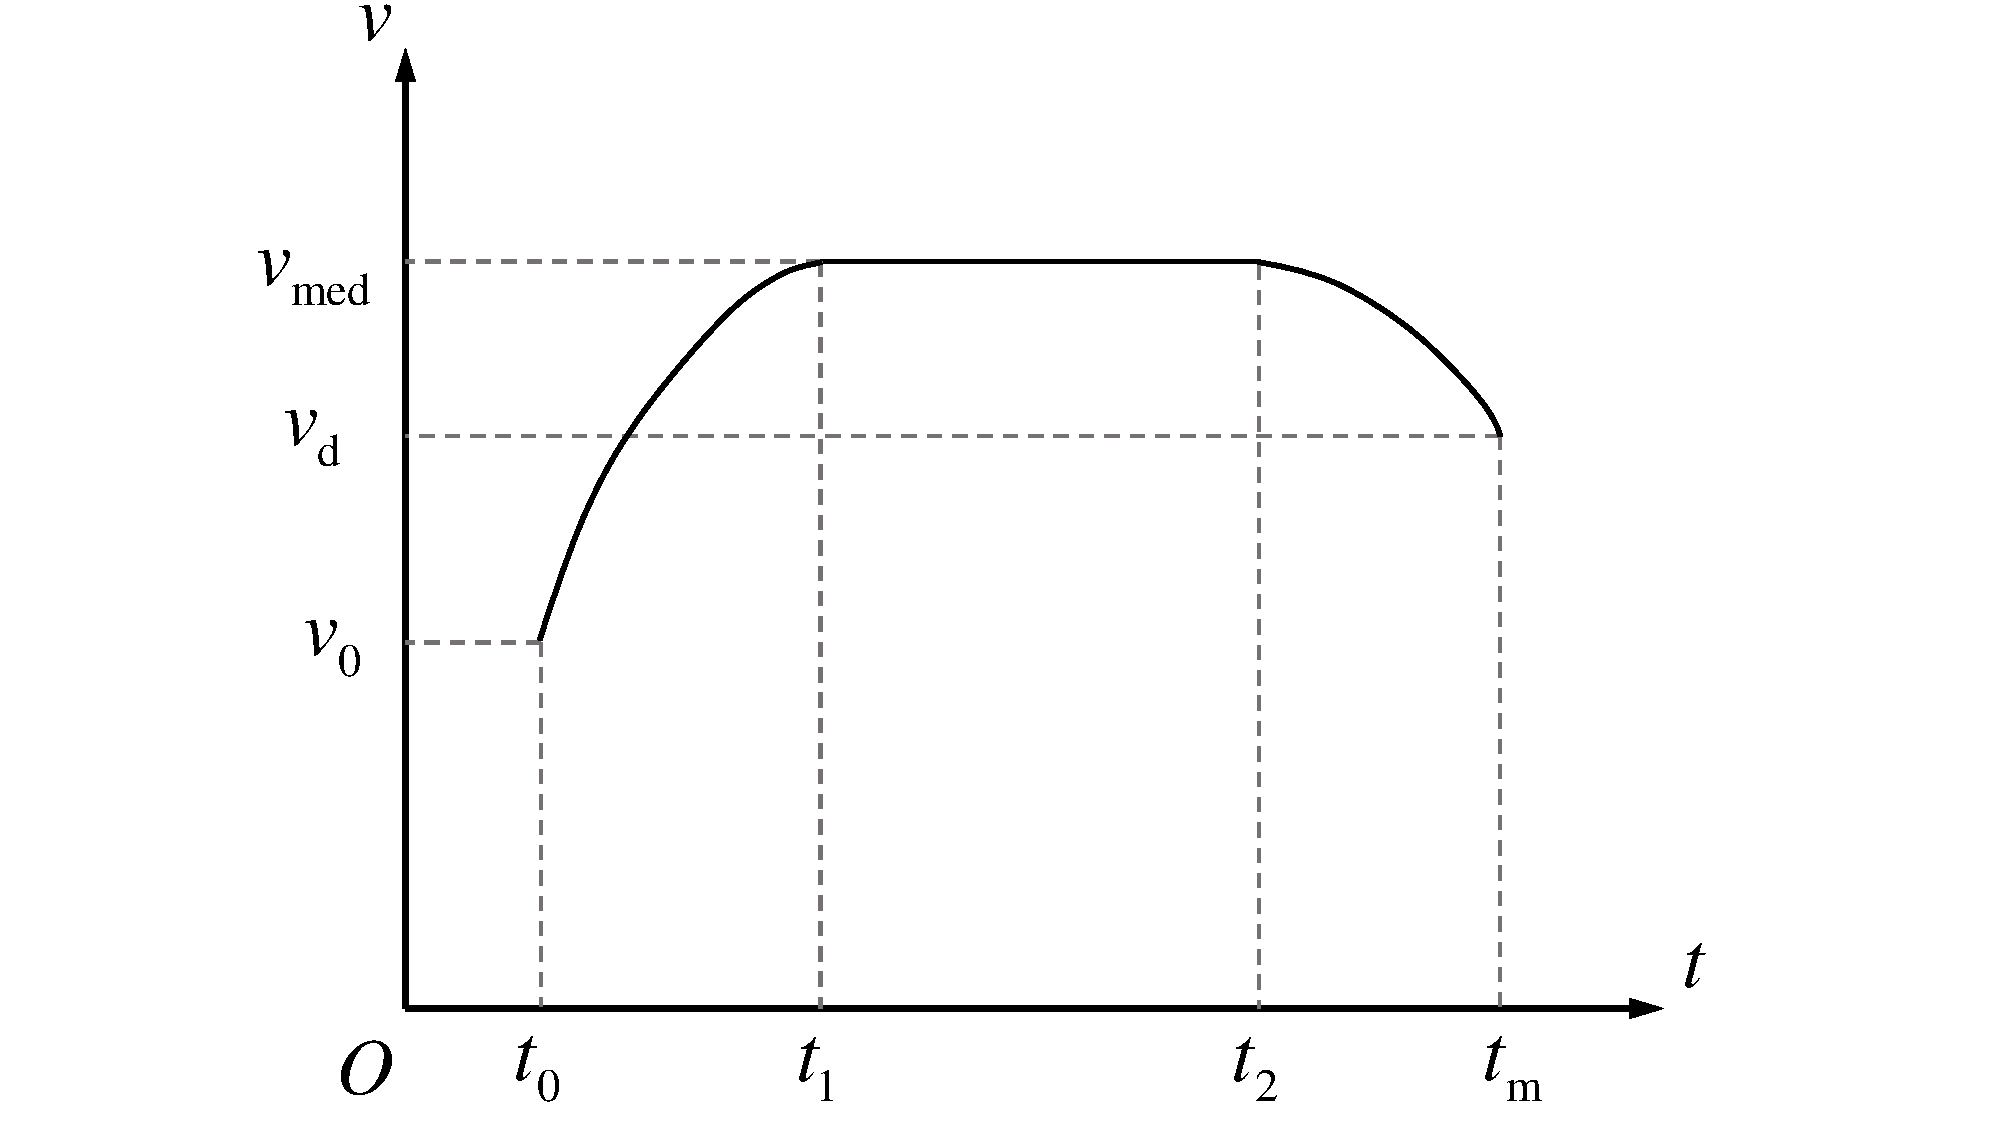
\includegraphics[width=12cm]{figures/vc.pdf}
\caption{速度约束下的速度-时间关系图}
\label{fig:vc}
\end{figure}

\begin{figure}[htbp]
\centering
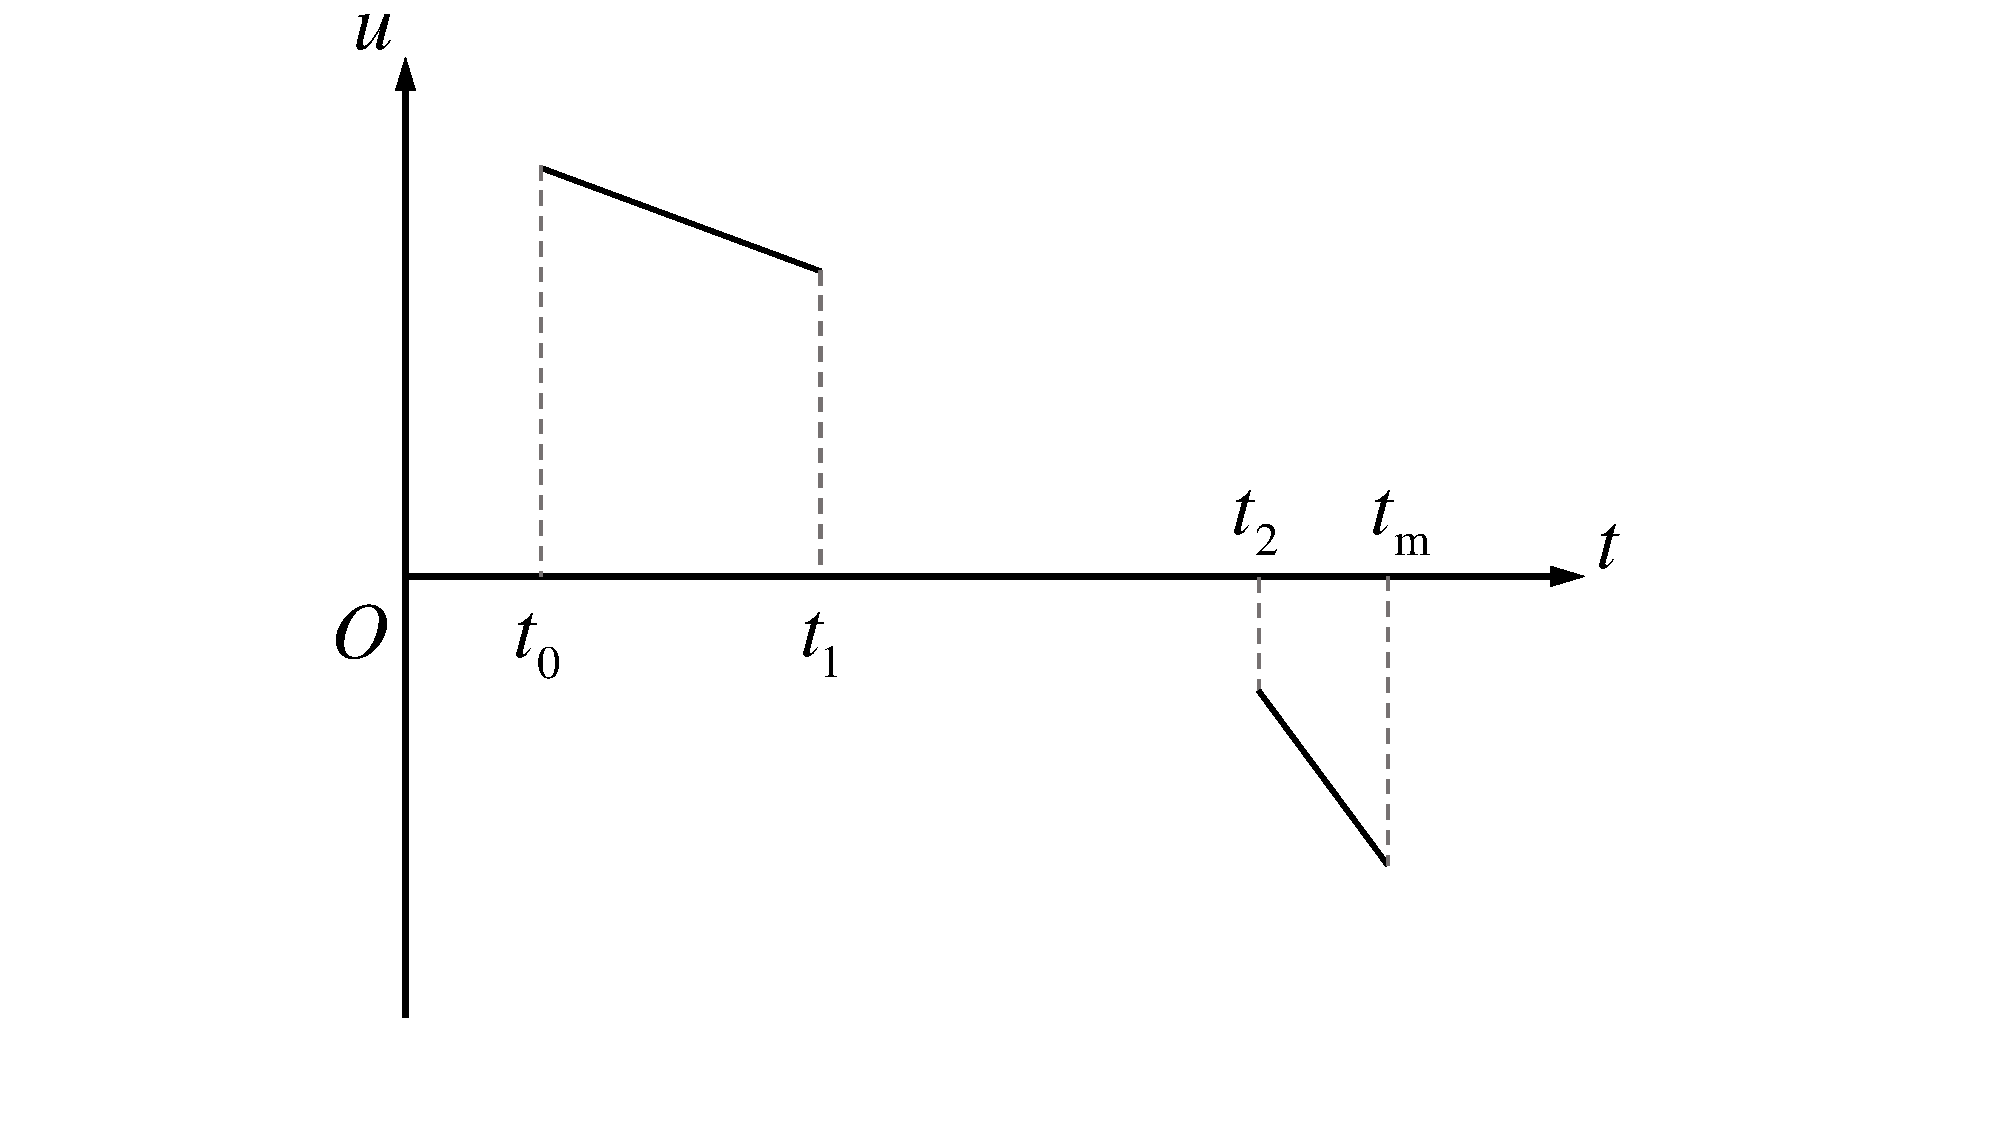
\includegraphics[width=12cm]{figures/vcu.pdf}
\caption{速度约束下的加速度-时间关系图}
\label{fig:vcu}
\end{figure}

基于以上的推断,将整个控制区的控制过程分为三段,分别为二次加速度段,匀速段和二次减速段。如图\ref{fig:vc}为速度与时间的关系图,图\ref{fig:vcu}为加速度与时间的关系图。这里“二次”是指速度为时间的二次函数。其中加速度的分段表达式为,
\begin{equation}
u(t)=
\begin{dcases}
a_1t+b_1,\quad& t_0\leq t < t_1,\\
0, \quad& t_1\leq t < t_2,\\
a_2t+b_2,\quad& t_2\leq t\leq t_\mathrm{m},
\end{dcases}
\end{equation}
其中,
\begin{gather}
a_1t+b_1 \geq 0,\quad \forall t\in [t_0,t_1),\label{eq:num:ac1}\\
a_2t+b_2 \leq 0,\quad \forall t\in [t_2,t_\mathrm{m}],\label{eq:num:ac2}\\
a_1\leq 0,\ a_2\leq 0.\label{eq:num:ac3}
\end{gather}
以上约束中式\eqref{eq:num:ac1}和\eqref{eq:num:ac2}保证了在第一段和第三段中,速度不出现峰值。可以这样考虑:如果在第一段速度出现一个极值后又下降,反而不如保持极值时的速度直接进入匀速段,不仅运行更快,而且省去了减速需要耗费的能量。同理第三段也应该只存在减速,而不能先加速再减速。式\eqref{eq:num:ac3}保证了第一、第三段的速度都是上凸的。可以这样考虑:假设$a_1>0$,可以将第一段加速度沿$u=a_1(t_0+t_1)/2+b_1$翻转,如图\ref{fig:uvert}所示。可以观察到二者所夹的面积是相同的,即速度的变化量是相同的。如图\ref{fig:vvert}在速度变化相同的情况下,上凸的速度显然比下凸的位移更多,因此最优控制下的速度一定是上凸的。对$a_2$的分析同理。
\begin{figure}[htbp]
\begin{minipage}{0.50\textwidth}
  \centering
  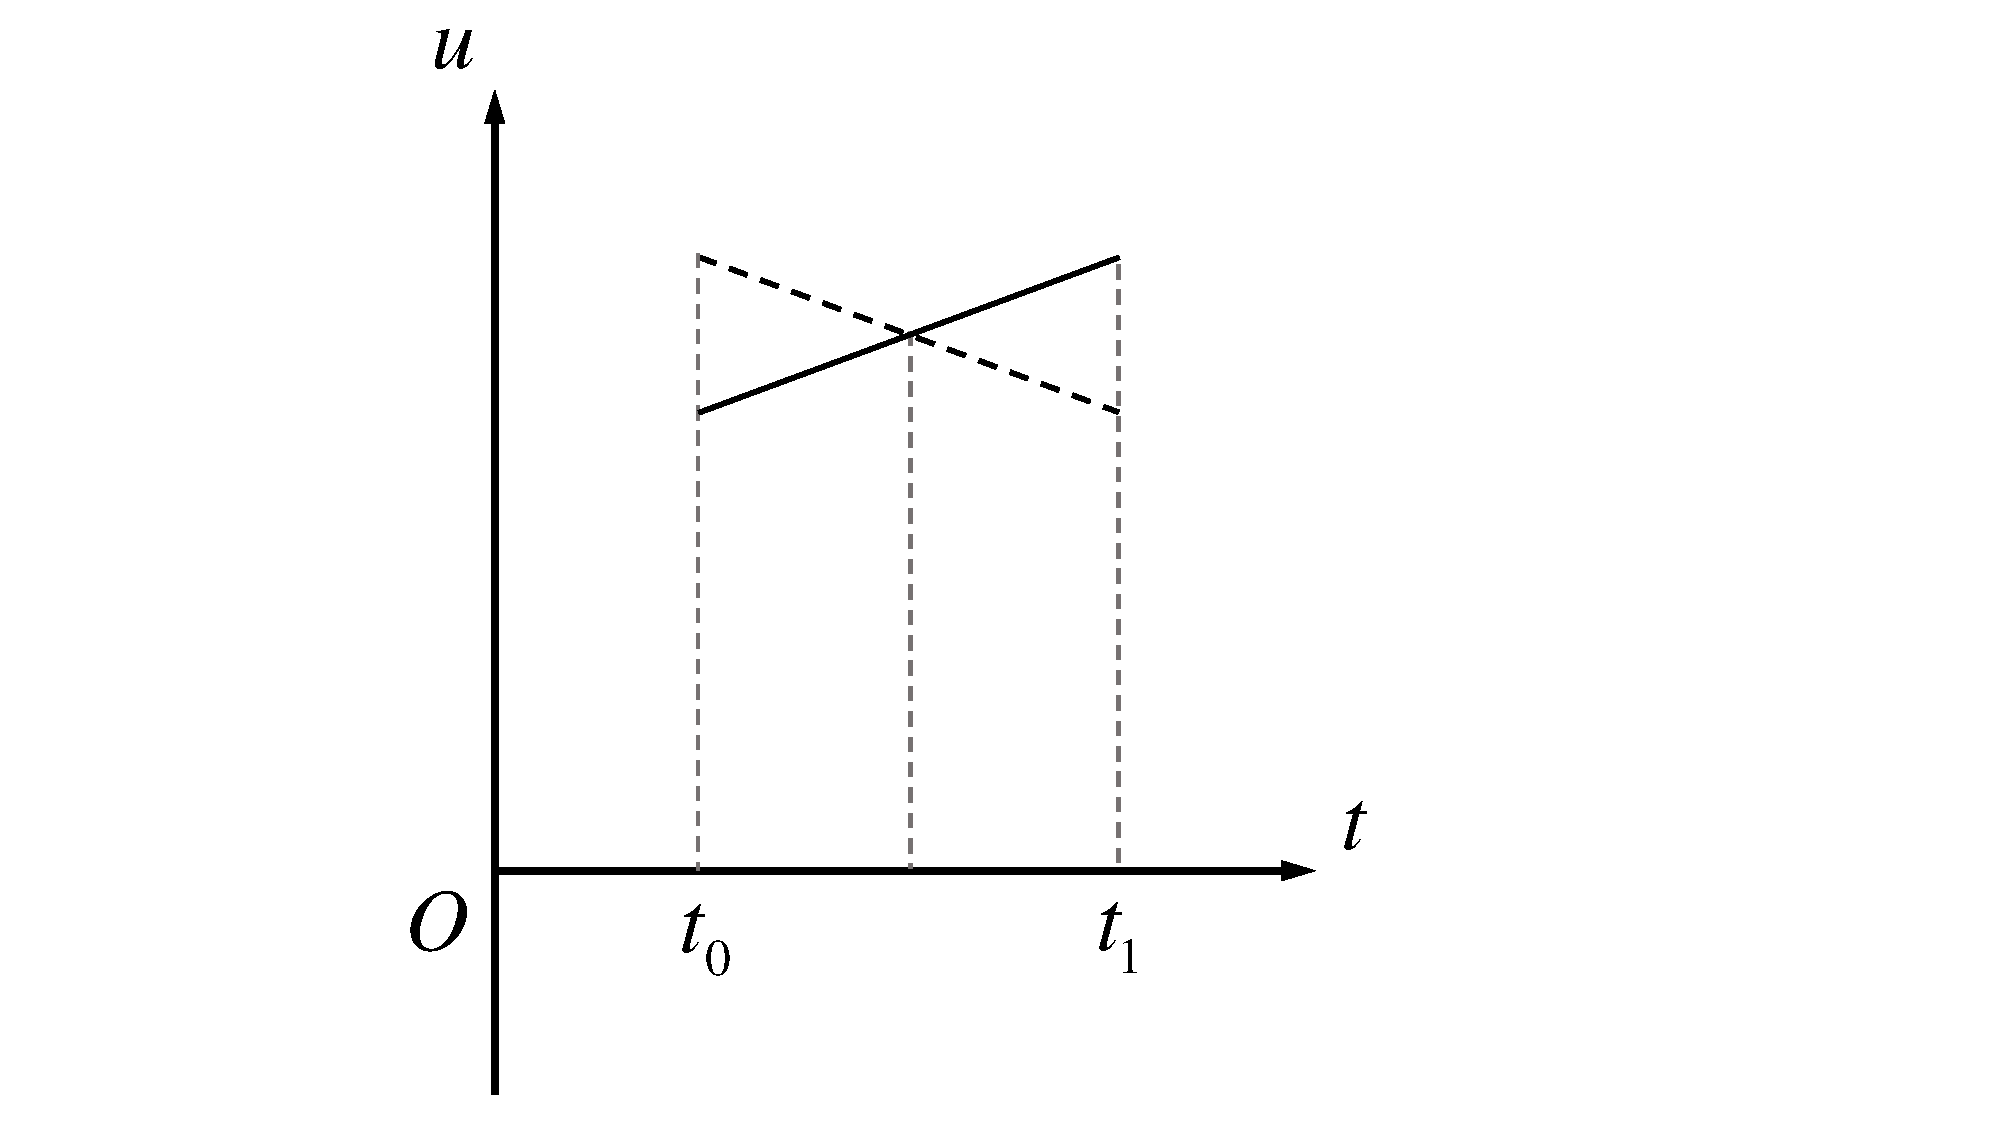
\includegraphics[height=8cm,trim={5cm 0 9cm 0},clip]{figures/uvert.pdf}
  \caption{加速度的翻转}
  \caption*{\small 实线为原加速度,虚线为翻转后加速度}
  \caption*{}
  \label{fig:uvert}
\end{minipage}\hfill
\begin{minipage}{0.45\textwidth}
  \centering
  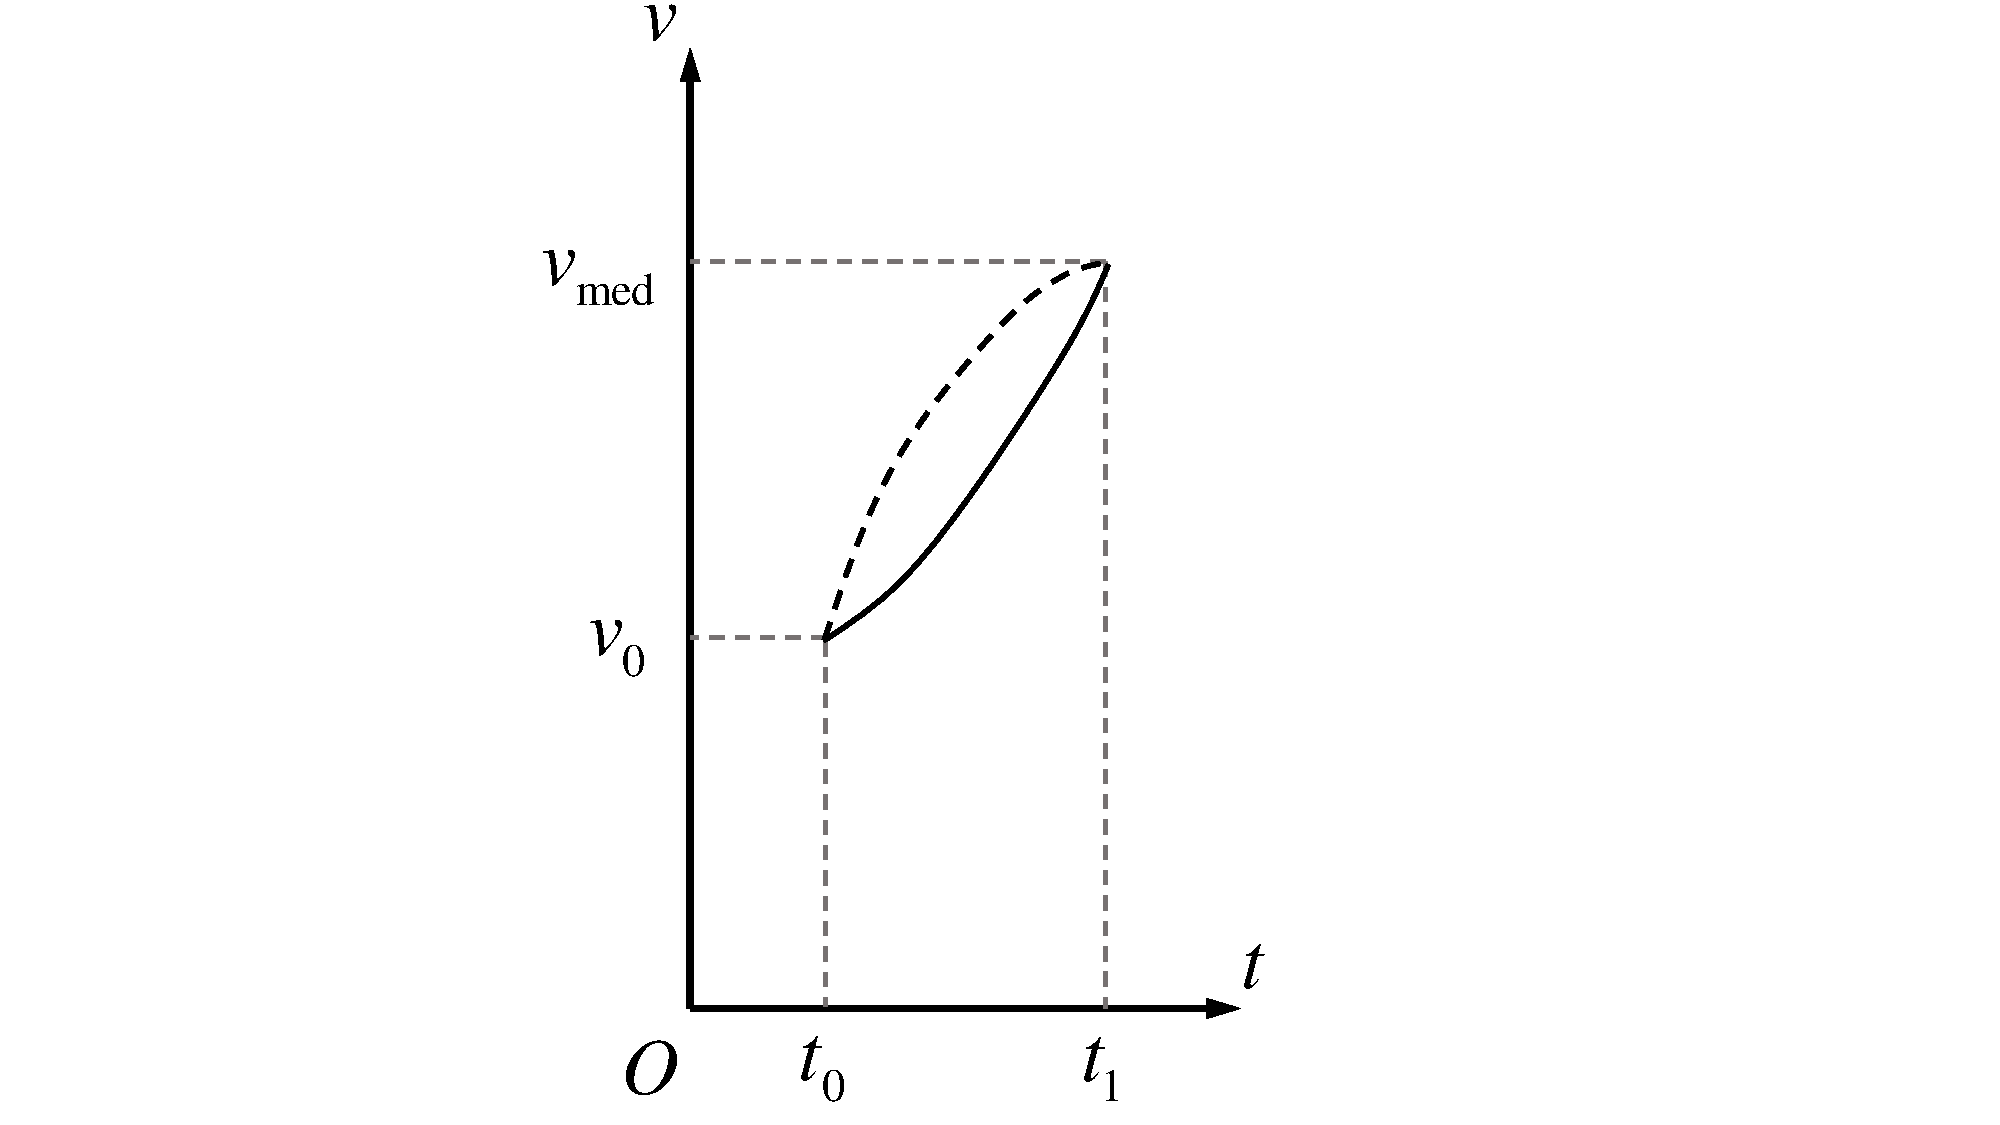
\includegraphics[height=8cm,trim={7cm 0 8cm 0},clip]{figures/vvert.pdf}
  \caption{速度的翻转}
  \caption*{实线为原加速度对应的速度,虚线为翻转后的加速度对应的速度}
  \label{fig:vvert}
\end{minipage}
\end{figure}

速度的分段表达式为,
\begin{equation}
v(t)=
\begin{dcases}
\frac12 a_1t^2+b_1t+c_1,\quad& t_0\leq t < t_1,\\
v_\mathrm{med}, \quad& t_1\leq t < t_2,\\
\frac12 a_2t^2+b_2t+c_2,\quad& t_2\leq t < t_\mathrm{m},
\end{dcases}
\end{equation}
其中,
\begin{equation}
v_\mathrm{med}\leq v_{\max}.
\end{equation}


\subsection{考虑速度与加速度约束}


% \begin{algorithm}
% \caption{最优通行时间顺序下的群决策算法}
% \begin{algorithmic}[1]
%   \Require{$x$ and $y$ are packed \DNA strings of equal length $n$}
%   \Statex
%   \Function{Distance}{$x, y$}
%     \Let{$z$}{$x \oplus y$} \Comment{$\oplus$: bitwise exclusive-or}
%     \Let{$\delta$}{$0$}
%     \For{$i \gets 1 \textrm{ to } n$}
%       \If{$z_i \neq 0$}
%         \Let{$\delta$}{$\delta + 1$}
%       \EndIf
%     \EndFor
%     \State \Return{$\delta$}
%   \EndFunction
% \end{algorithmic}
% \end{algorithm}
% \section{算法可行性分析}

% \subsection{时间序列可行性}
% \subsection{控制区不碰撞的证明}